\chapter{\IfLanguageName{dutch}{Stand van zaken}{State of the art}}%
\label{ch:stand-van-zaken}

% Tip: Begin elk hoofdstuk met een paragraaf inleiding die beschrijft hoe
% dit hoofdstuk past binnen het geheel van de bachelorproef. Geef in het
% bijzonder aan wat de link is met het vorige en volgende hoofdstuk.

% Pas na deze inleidende paragraaf komt de eerste sectiehoofding.

\section{Network and Information Security 2}%
\label{sec:nis2}

\section{Huidige aanpak van asset management}%
\label{sec:huidige_aanpak_van_asset_management}

\subsection{Infrastructure as Code}%
\label{sub:ias}

\subsection{Data Center Infrastructure Management}
\label{sub:dcim}

\subsection{IP Address Management}
\label{sub:ipam}

\subsection{Snipe-IT}
\label{sub:snipe-it}

Snip-IT is een open-source webapplicatie ontwikkeld door Grokability sinds 2013~\autocite{snipe-it-introduction}, die gericht is op IT-assetmanagement.
Het idee achter Snipe-IT komt voort uit de vroegere aanpak van het bedrijf, toen het voornamelijk nog gebruik maakte van spreadsheets om hun bedrijfsmiddelen te inventariseren.
Het doel was om een applicatie te ontwikkelen die deze taak op een meer georganiseerde en effici\"ente manier kon uitvoeren.

\begin{figure}[h!]
    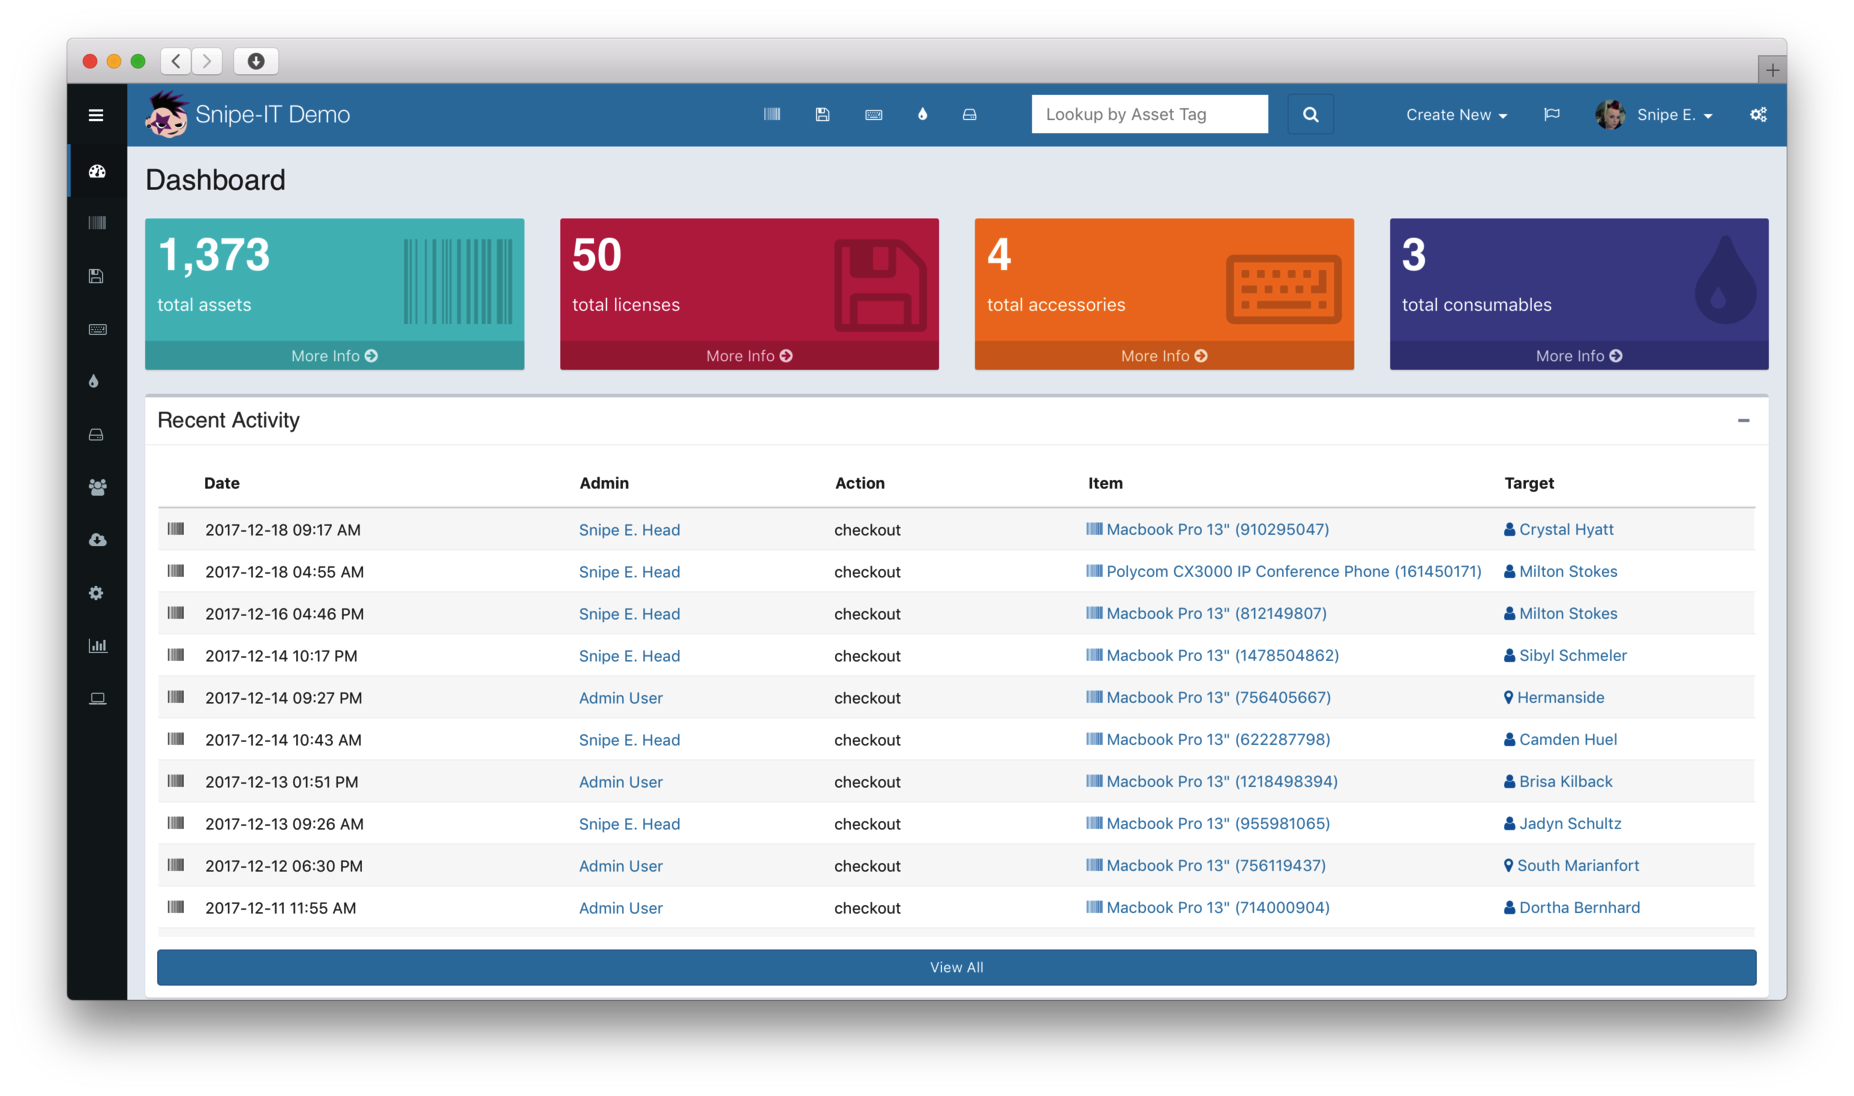
\includegraphics[width=\textwidth]
    {./graphics/snipe-dashboard.png}
    \caption{\label{fig:snipe-it-dashboard}Snip-IT dashboard.}
\end{figure}

De software biedt een gebruiksvriendelijke webinterface (\ref{fig:snipe-it-dashboard}) waarmee bedrijfsmiddelen, licenties, garanties en meer gemakkelijk kunnen worden beheerd.
Wanneer men kiest voor de self-hosted optie is de software gratis beschikbaar, terwijl ook verschillende cloud-gebaseerde optie beschikbaar zijn tegen een jaarlijkse bijdrage.
Deze prijs varieert afhankelijk van de nodige features en support.
Alle code en services gerelateerd aan Snipe-IT zijn vrij beschikbaar op GitHub~\autocite{snipe-it-github}.

Enkele van de belangrijkste functies van Snipe-IT zijn~\autocite{snipe-it-features}, maar zijn niet beperkt tot:
\begin{itemize}
    \item Het eenvoudig bekijken van toegewezen bedrijfsmiddelen, inclusief informatie over wie ze gebruikt en hun fysieke locatie.
    \item Het groeperen van gemeenschappelijke functies met behulp van Asset Models.
    \item E-mailwaarschuwingen voor het verstrijken van garanties en licenties.
    \item Snelle en eenvoudige controle van bedrijfsmiddelen.
    \item Het gemakkelijk importeren en exporteren van assets.
\end{itemize}

\subsection{Nagios}
\label{sub:nagios}

\subsection{Lansweeper}
\label{sub:lansweeper}
